\section{Measurement Pitfalls}
\label{sec:measurement}

A placement experiment claims that a latency difference was caused by the
choice of backup. Each subsection below describes one way that claim fails, the
evidence, and the control adopted in \S\ref{sec:results}.

\subsection{The RPC Stack Biases the Measured Effect}
\label{sec:p99}

DEFT's \texttt{Backup} is a \texttt{SimpleXMLRPCServer}: single-threaded,
HTTP/1.0, listening with a backlog of five. HTTP/1.0 means the server closes the
connection after each response, so every replication call performs a fresh TCP
handshake. We verified this directly: twenty calls through one client proxy
produce twenty server-side \texttt{accept()}s.

\textbf{The latency tail is a kernel timer.} Under burst load the five-deep
backlog overflows, the SYN is dropped, and the client waits out the kernel's
retransmission timer. On the single-machine harness at 16 hosts the resulting
distribution is bimodal with an empty gap between the modes: $82.3\%$ of calls
complete under $100$\,ms and $3.2\%$ beyond $900$\,ms, while the
$500$--$900$\,ms band holds $0.042\%$. The slow calls sit at
$1052$--$1059$\,ms with a standard deviation of 24--29\,ms at every scale, which
is Linux's initial SYN-retransmission timeout; the next retry contributes a
cluster near 3\,s. On this transport p99 is therefore a threshold statistic: it
reads tens of milliseconds or about $1050$\,ms depending only on whether a run's
SYN-drop rate crosses one percent.

\textbf{A persistent-connection transport has no such tail.}
Figure~\ref{fig:tailtransport} plots the complementary CDF of per-call latency
for the same workload over XML-RPC and over our gRPC implementation
(180{,}000 and 300{,}000 calls). The XML-RPC curve is a staircase that steps
down at each timer quantum, with $3.20\%$ of calls beyond 900\,ms and a maximum
of 22{,}773\,ms. The gRPC curve decays smoothly, with $0.013\%$ beyond 900\,ms
and a maximum of 1139\,ms. On the same harness the measured advantage of the
heuristic over \texttt{round\_robin} is about four times larger on XML-RPC than
on gRPC ($48.05$ against $11.43$\,ms at 16 hosts, $43.69$ against $9.75$ at 32):
a degraded host's added service time pushes its accept queue into overflow,
which converts a modest penalty into seconds of retransmission wait. The two
arms differ in more than the connection model, however, so this comparison
motivates the direct test and does not replace it.

\begin{figure}[t]
\centering
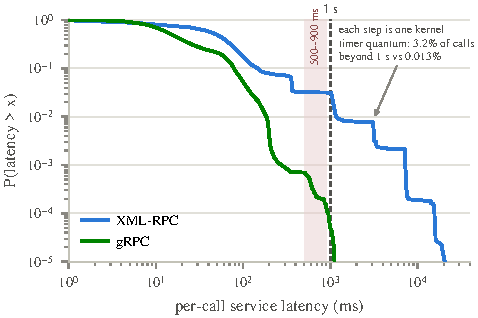
\includegraphics[width=\columnwidth]{figures/fig_tail_transport.pdf}
\caption{Complementary CDF of per-call service latency at 16 hosts on the
single-machine harness, by transport (log--log). The XML-RPC tail is a staircase
of kernel timer quanta; the gRPC tail decays smoothly and ends two orders of
magnitude earlier. The shaded band is 500--900\,ms.}
\label{fig:tailtransport}
\end{figure}

\textbf{The accept queue, tested directly.} On the bare-metal testbed we hold
everything fixed, change only the listen backlog, and read the kernel's
counters. With the shipped backlog of five and all 128 hosts healthy, four
methods whose p95 differs by less than $2$\,ms have p99 values within $12$\,ms
of $1040$\,ms. A constant that survives every change of method is an artifact.
The counters confirm the mechanism: $103{,}209$ \texttt{ListenOverflows} on the
most heavily selected node against $116$ retransmitted segments, with
\texttt{ListenDrops} equal to \texttt{ListenOverflows}. The connections were
refused at the server, not lost in the network. Raising the backlog to $512$
drove the overflow count to zero and p99 from $1040$\,ms to $79$\,ms.

% Generated by make_testbed_tables.py -- do not edit by hand.
\begin{table}[t]
\centering
\caption{Mean service latency against the number of primaries sharing a backup, homogeneous hosts. The steep response under the shipped backlog is dropped SYNs and the client's 1\,s retransmission timeout, not queueing at the backup. Milliseconds.}
\label{tab:loadcurve}
\begin{tabular}{rrr}
\toprule
Primaries sharing & Backlog 5 & Backlog 512 \\
\midrule
1 & 50.3 & 41.9 \\
2 & 54.4 & 41.0 \\
4 & 75.0 & 41.3 \\
16 & 219.0 & 42.4 \\
45 & 342.6 & 49.7 \\
79 & 378.2 & 56.4 \\
\bottomrule
\end{tabular}
\end{table}


\textbf{What sharing a backup costs.} Table~\ref{tab:loadcurve} gives mean
latency against the number of primaries sharing one backup, with homogeneous
hosts. Under the shipped backlog latency rises $7.5\times$ from one primary per
backup to seventy-nine. With a backlog of 512 the same sweep costs $35\%$, and
up to sixteen primaries on one backup it costs under $1$\,ms. Most of the
apparent penalty for concentration was connection setup being refused and not
queueing at the backup. This has a consequence beyond the artifact: on this
testbed, with a backup that does no work per call (\S\ref{sec:sut}), moderate
sharing is nearly free, which is why we do not read small differences in peak
load as latency differences (\S\ref{sec:scenarios}) and why degraded-host
exposure, not load balance, accounts for the effect in \S\ref{sec:hetero}.

% Generated by make_testbed_tables.py -- do not edit by hand.
\begin{table}[t]
\centering
\caption{DEFT's accept backlog as the only variable, 16 hosts on bare metal with identical \texttt{tc netem} degradation. The five-deep queue sheds load rather than queueing it, which lowers the median and produces the one-second tail. Milliseconds.}
\label{tab:backlog16}
\resizebox{\columnwidth}{!}{%
\begin{tabular}{lrrrrrr}
\toprule
& \multicolumn{3}{c}{Backlog 5 (as shipped)} & \multicolumn{3}{c}{Backlog 512} \\
\cmidrule(lr){2-4}\cmidrule(lr){5-7}
Method & Mean & Median & p99 & Mean & Median & p99 \\
\midrule
\texttt{optimal} & 28.70 & 14.64 & 1015.26 & 23.17 & 22.68 & 49.45 \\
\texttt{heuristic} & 32.04 & 12.08 & 1020.77 & 23.82 & 23.09 & 56.76 \\
\texttt{round\_robin} & 35.22 & 14.44 & 1013.35 & 29.89 & 22.11 & 120.62 \\
\texttt{random} & 51.54 & 12.04 & 858.46 & 36.45 & 23.62 & 95.39 \\
\texttt{PPO} & 32.46 & 11.13 & 1022.93 & 23.49 & 22.87 & 49.84 \\
\texttt{concentrated} & 101.70 & 101.49 & 104.30 & 101.71 & 101.52 & 104.52 \\
\bottomrule
\end{tabular}}
\end{table}


\textbf{The bias does not have a single sign.} Repeating the 16-host scenario
on the same nodes with the same \texttt{tc} degradation, changing only the
backlog, gives the opposite result (Table~\ref{tab:backlog16}). The one-second
plateau appears as before, with p99 of $1013$--$1023$\,ms across four methods
whose p95 spans $28$ to $102$\,ms. But the gap between methods is
\emph{larger} once the backlog is raised: \texttt{round\_robin} minus
\texttt{heuristic} is $3.18$\,ms as shipped and $6.07$\,ms at backlog 512. At
this scale the shipped queue understates the placement effect.

The two results are consistent once the mechanism is stated. Overflow is driven
by how many primaries share one backup. At 128 hosts with 80 primaries,
concentration is extreme and the overflow penalty falls hardest on the
placements that are already worst, which exaggerates the spread. At 16 hosts
with 10 primaries nothing is concentrated enough for that, so the penalty falls
roughly evenly and compresses the spread. The shipped backlog therefore biases
a measured placement effect with a sign that depends on how concentrated the
workload is, and no constant correction removes it.

The same table shows a property of the shipped configuration itself: the
five-deep queue \emph{lowers} the median, from $22.68$ to $14.64$\,ms for
\texttt{exact}. A short accept queue is admission control. Accepted calls
contend with fewer others at a single-threaded server and complete faster;
refused calls wait a full second.

\textbf{Control adopted.} Every bare-metal placement run uses a backlog of 512,
and p99 is reported only there. Any placement study over connection-per-call
RPC is subject to the same bias.

\subsection{How a Degraded Host Is Made Slow, and Where It Sits}
\label{sec:degconstruct}

\textbf{Degradation is imposed by the kernel.} A delay slept inside the server
measures a model of degradation, so the testbed slows hosts physically.
\texttt{tc netem} attaches to an interface, but a node here carries thirteen
backups and shaping the interface would also slow the healthy co-tenants that
the comparison needs as controls. Each backup owns a distinct TCP port, so a
\texttt{prio} qdisc with a \texttt{u32} filter on source port delays exactly
the degraded servers. The fourth band of a four-band \texttt{prio} is
unreachable through the default priomap, so healthy flows never enter the netem
queue. Measured on adjacent ports of one interface, a degraded backup costs
$101.4$\,ms per call and its healthy neighbour $1.0$\,ms. The $101.4$ is itself
informative: \texttt{netem} delays every packet the server sends, so a
connection-per-call protocol pays the added delay twice, on the SYN-ACK and on
the response.

\textbf{A contiguous degraded block makes order-based baselines look better
than they are.} With the sixteen degraded hosts chosen as a contiguous block of
names, \texttt{w81}--\texttt{w96}, \texttt{round\_robin} ties with
\texttt{exact} at $41.3$\,ms and selects a degraded host $0\%$ of the time. The
tie is an artifact of naming. \texttt{round\_robin} cycles a lexicographically
sorted host list in which every name beginning \texttt{w1}--\texttt{w7}
precedes \texttt{w8}; with 80 primaries the cursor advances 80 positions and
never reaches the block. The method scores zero by never arriving. Spreading
the same sixteen hosts evenly along that ordering puts them within every
method's reach, after which \texttt{round\_robin} meets them at the base rate
and its mean rises from $41.28$ to $51.87$\,ms. The same layout dependence
appears in a learned policy that has collapsed onto two hosts
(\S\ref{sec:rl128}).

\textbf{Control adopted.} Degraded hosts are spread evenly through the host
ordering in every bare-metal run and redrawn at random per seed in every
structural comparison (Tables~\ref{tab:terms} and~\ref{tab:hrw}), and every
latency table reports the share of each method's calls that reached one. Without that
column the latency comparison cannot be interpreted.

\subsection{A Degradation Model That Cannot Rank Scoring Functions}
\label{sec:binarymodel}

The previous subsection concerns how a degraded host is made slow. This one
concerns how it is made visible to the selector. Under the binary model a
degraded host has health $0.05$ against a healthy draw from $[0.5, 1.0]$ and a
capacity ratio of $0.033$ against $1.0$: an order of magnitude away on both
host features of the score, and identical to every other degraded host. We ran
the sweep of \S\ref{sec:weights} under that model at the three scales. Every
configuration with any weight on health or on capacity, 275 of the 286,
assigns no degraded backup in any of 30 seeds. A weight of $0.1$ on either
term is as good as $1.0$, so the model cannot say which weighting is better,
or which term matters.

\textbf{A fixed layout hides even that.} In an earlier form of the sweep the
degraded hosts were the same in every seed. The remaining 11 configurations,
which read no host state and give every primary the same backup, then also
scored zero, because the host they all select was never among the degraded
ones. A benchmark in which a score that reads nothing is perfect measures the
layout. With the degraded hosts redrawn per seed those configurations meet
them at about the base rate, as they should.

\textbf{Control adopted.} We use the binary model only where its purpose is to
make degraded hosts unmistakable, to measure what selecting one costs
(\S\ref{sec:hetero}), and we say so. Claims about which signal detects
degradation rest on the realistic model, with layouts, failure kinds and
severities redrawn per seed and a signal-blind configuration reported as the
reference (\S\ref{sec:weights}).
